\documentclass[]{finalproject}
\usepackage[algoruled, linesnumbered, noline]{algorithm2e}
\usepackage{float}
\usepackage{graphicx}
\usepackage{minted}
\usepackage{ragged2e}
\graphicspath{{./img}}

\usepackage{parskip}
\usepackage{float}
\usepackage{wrapfig}

\captionsetup{labelfont={bf}}

% Title (and subtitle) of the project
\title{Quicksort}
\subtitle{}

% Group members for the final project (comment out the unnecessary entries)
\begin{groupmembers}
\studentA{Pratyai}{}{Mazumder}
\studentB{Lodovico}{}{Mazzei}
\studentC{Michele}{}{Chersich}
\end{groupmembers}

\abstract {
A short abstract summarising what your project is about and the main results you obtained.
}


\begin{document}
\maketitle

\section{Introduction} \label{introduction}
\subsection{The sorting problem}

\section{The algorithm}


\subsection{The partitioning problem}

Quicksort belongs to the family of \textit{partition sort} algorithms,
where a partitioning routine is called recursively until a whole sequence is sorted.

Given an array $A[1,.....,N]$, the partitioning algorithm should split a permutation
of it, $A'$, into two partitions $U=A'[1,.....,p]$ and $V=A'[p+1,.....,N]$ such that
$U[i] \leq V[j] \;\, \forall \; i,j \in \{[1,p] , [p+1,N]\}$. 
By recursively partitioning U and V themselves, base cases will eventually be reached,
consisting of single-element or empty arrays, which are already sorted.
Figure \ref{fig:rec-part} illustrates the recursive routine.

\begin{figure}[H]
    \centering
    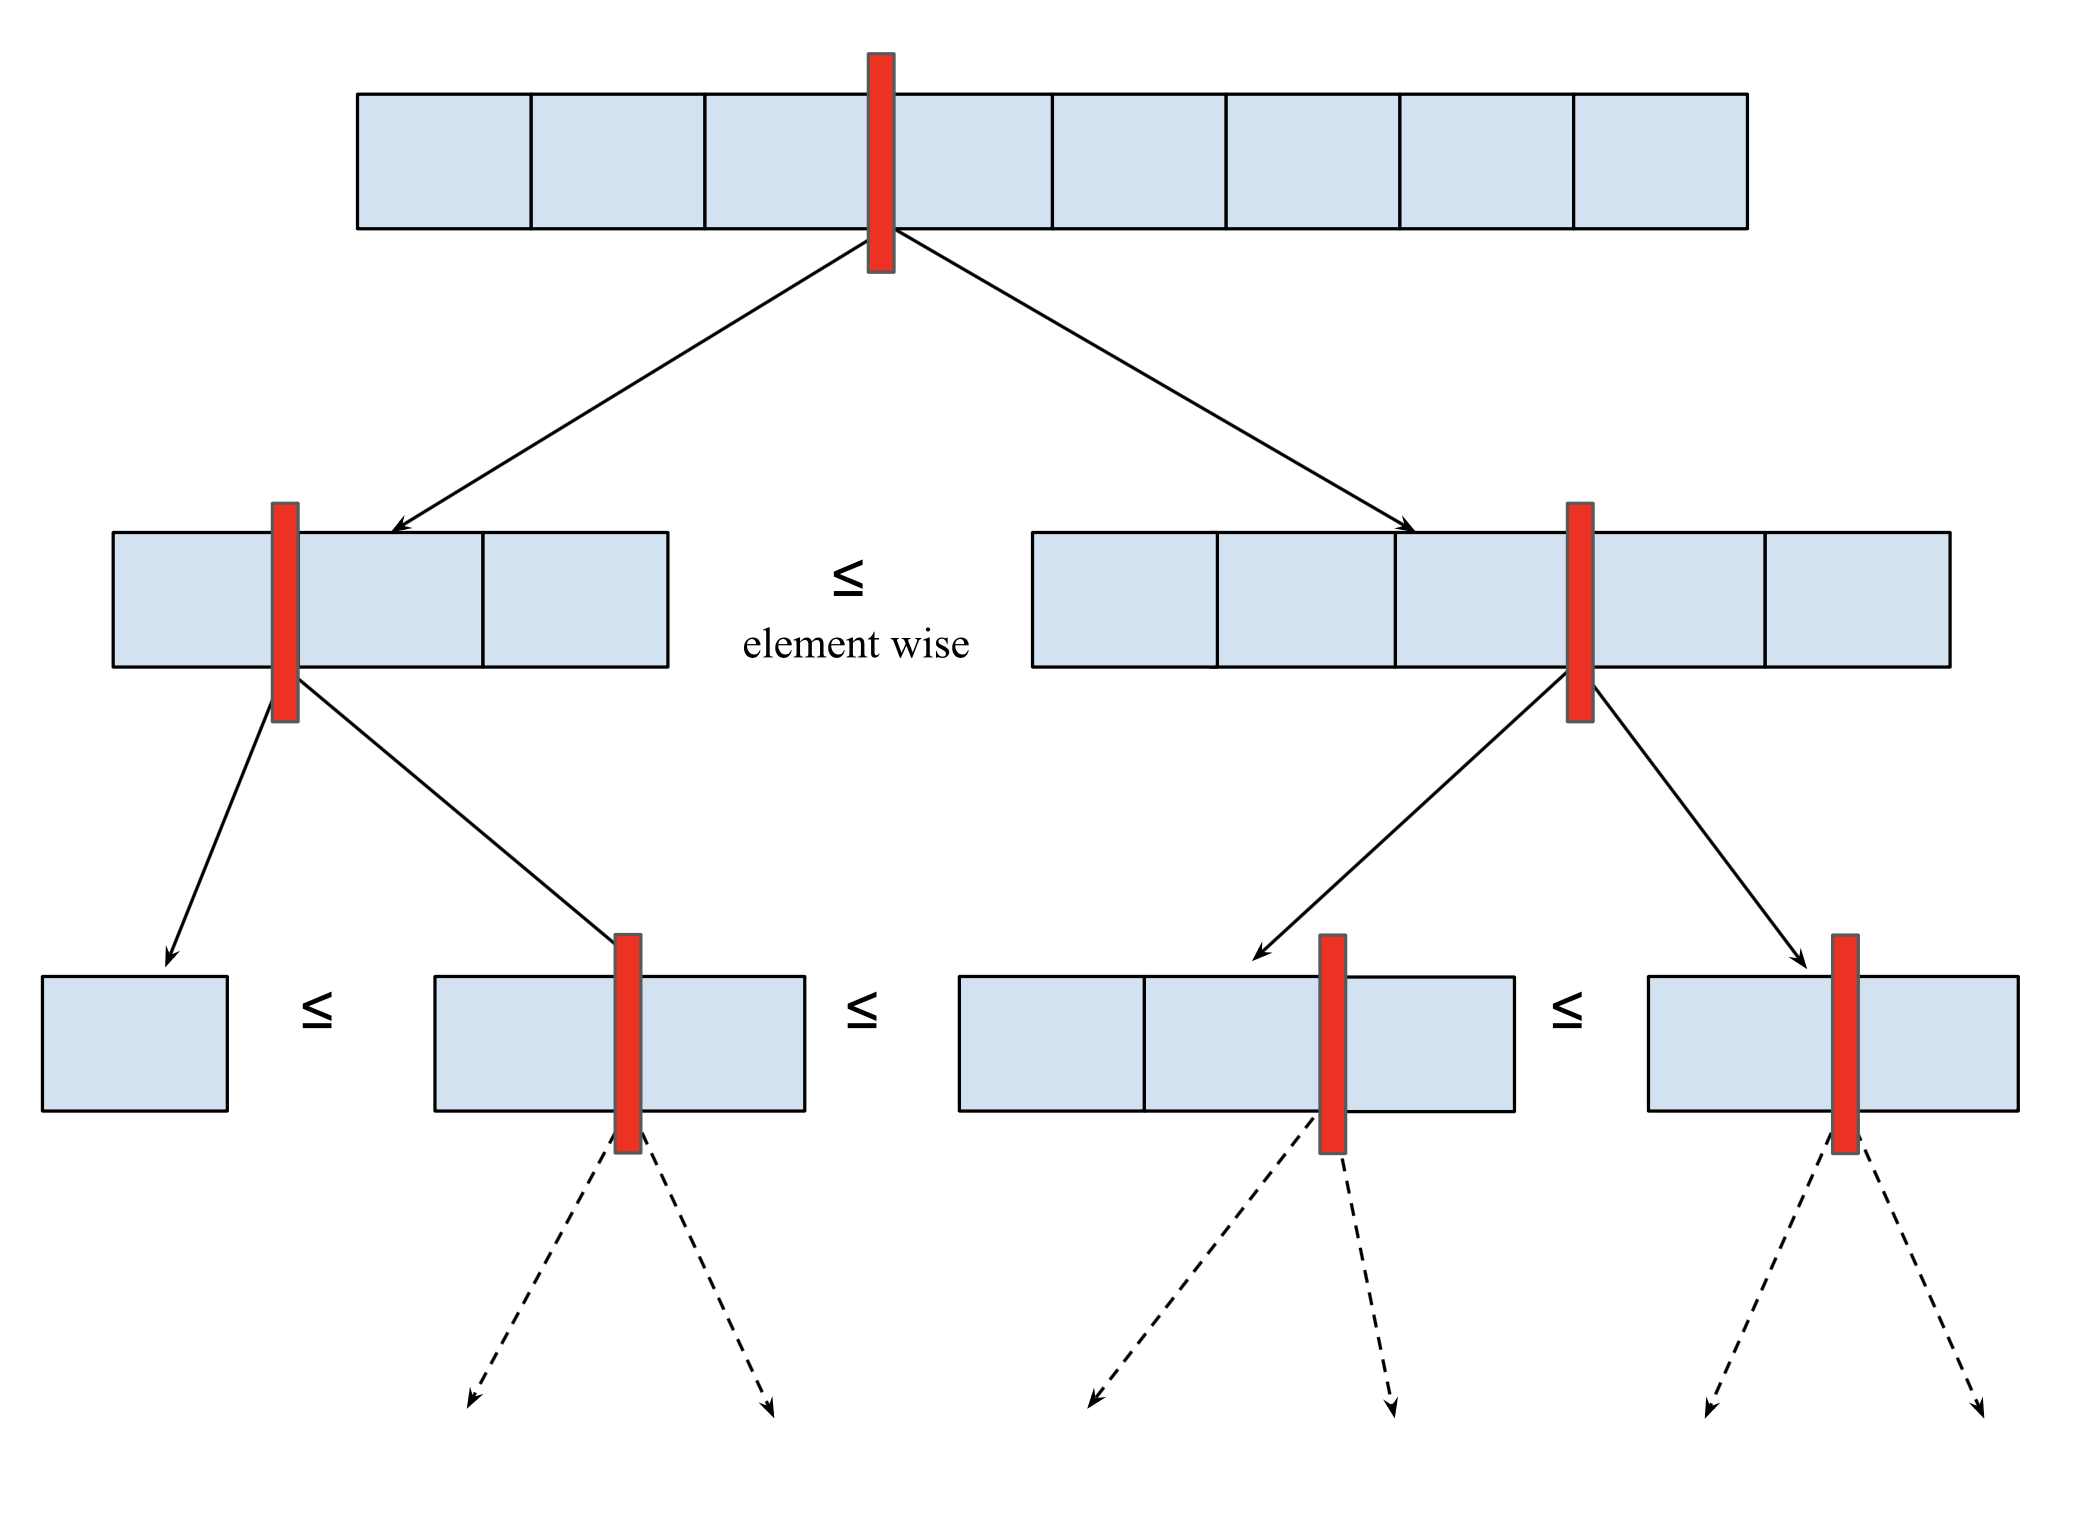
\includegraphics[width=0.6\textwidth]{recursive_partitioning.png}
    \caption{A picture of the same tucan looking the other way!A picture of the same tucan looking the other way!A picture of the same tucan looking the other way!A picture of the same tucan looking the other way!A picture of the same tucan looking the other way!A picture of the same tucan looking the other way!A picture of the same tucan looking the other way!A picture of the same tucan looking the other way!A picture of the same tucan looking the other way!A picture of the same tucan looking the other way!A picture of the same tucan looking the other way!}
    \label{fig:rec-part}
\end{figure}

The following pseudocode recursively sorts a given subarray of $A$. It assumes a partition routine which will be discussed in the following sections.

\begin{verbatim}
quicksort(A, low, high):
      if low >= 0 && high >= 0 && low < high then
            // Reorder A around the pivot in-place such that
            // the partition A[low],...,A[p] is pointwise
            // less than or equal to the partition A[p+1],...,A[high]
            p := partition(A, low, high)
            // Recursively solve the two partitions without affecting the partition invariant
            quicksort(A, low, p)
            quicksort(A, p+1, high)
\end{verbatim}

\subsection{Pivot selection}
The partitioning in quicksort relies on a method called pivoting. This consists in picking a value $\gamma$ to be our pivot. Given the array $A$, we then permute it in a way such that every element before $\gamma$ is smaller than it, and every one after it is larger. The internal order in these subarrays is irrelevant, as it will be addressed in further iterations of the algorithm.\\
Clearly, the pivot choice will have an impact on the efficiency of the algorithm. We divide the selection methods into two categories: one-step and multi-step.\\
The following paragraphs provide a description using as an example the array $A[1,.....,N]$ introduced above.

\subsubsection{One-step selection}
These methods only require chosing a value at each iteration and using it as the pivot, the difference being the position of $A$ from which the value is selected.

\begin{itemize}
\item{\textit{First element}}: set the pivot to be the value $A[1]$.
\item{\textit{Last element}}: set the pivot to be the value $A[N]$.
\item{\textit{Central element}}: set the pivot to be the value $A[\lfloor \frac{(N+1)}{2} \rfloor]$ or $A[\lceil \frac{(N+1)}{2} \rceil]$ if N is even, and $A[\frac{N+1}{2}]$ if N is odd.
\item{\textit{Random element}}: set the pivot to be value $A[r]$, where $r$ is a random number such that $1 \leq r \leq N$.
\end{itemize}

\subsubsection{Multi-step selection}
Given that the most efficient case of the partitioning is achieved when picking the median, the following methods involve computing the median of some odd sample of values extracted from the array. The difference among the methods lies in the positions of the array from which the values are taken, and in the sample size. The latter is indicated by the suffix $T$, with most common implementations using $3 \leq T \leq 9$

\begin{itemize}
\item{\textit{Median-of-T with fixed selection:}} $T$ integers $1 \leq n_{1},....,n_{T} \leq N$ are fixed beforehand. The median of $\{A[n_{1}],.....,A[n_{T}]\}$ is then computed and used as the pivot for the partitioning.
\item{\textit{Median-of-T with random selection:}} $T$ random integers $1 \leq r_{1},....,r_{T} \leq N$ are generated. The median of $\{A[r_{1}],.....,A[r_{T}]\}$ is then computed and used as the pivot for the partitioning.
\end{itemize}

\subsection{Partitioning around the pivot}
mention two main schemes
Figure 2 illustrates the process of partitioning around a chosen value, 4 in this case. Recalling the previous paragraph, this could have been a one-step selection using a random index.




\begin{figure}[H]
  \begin{center}
   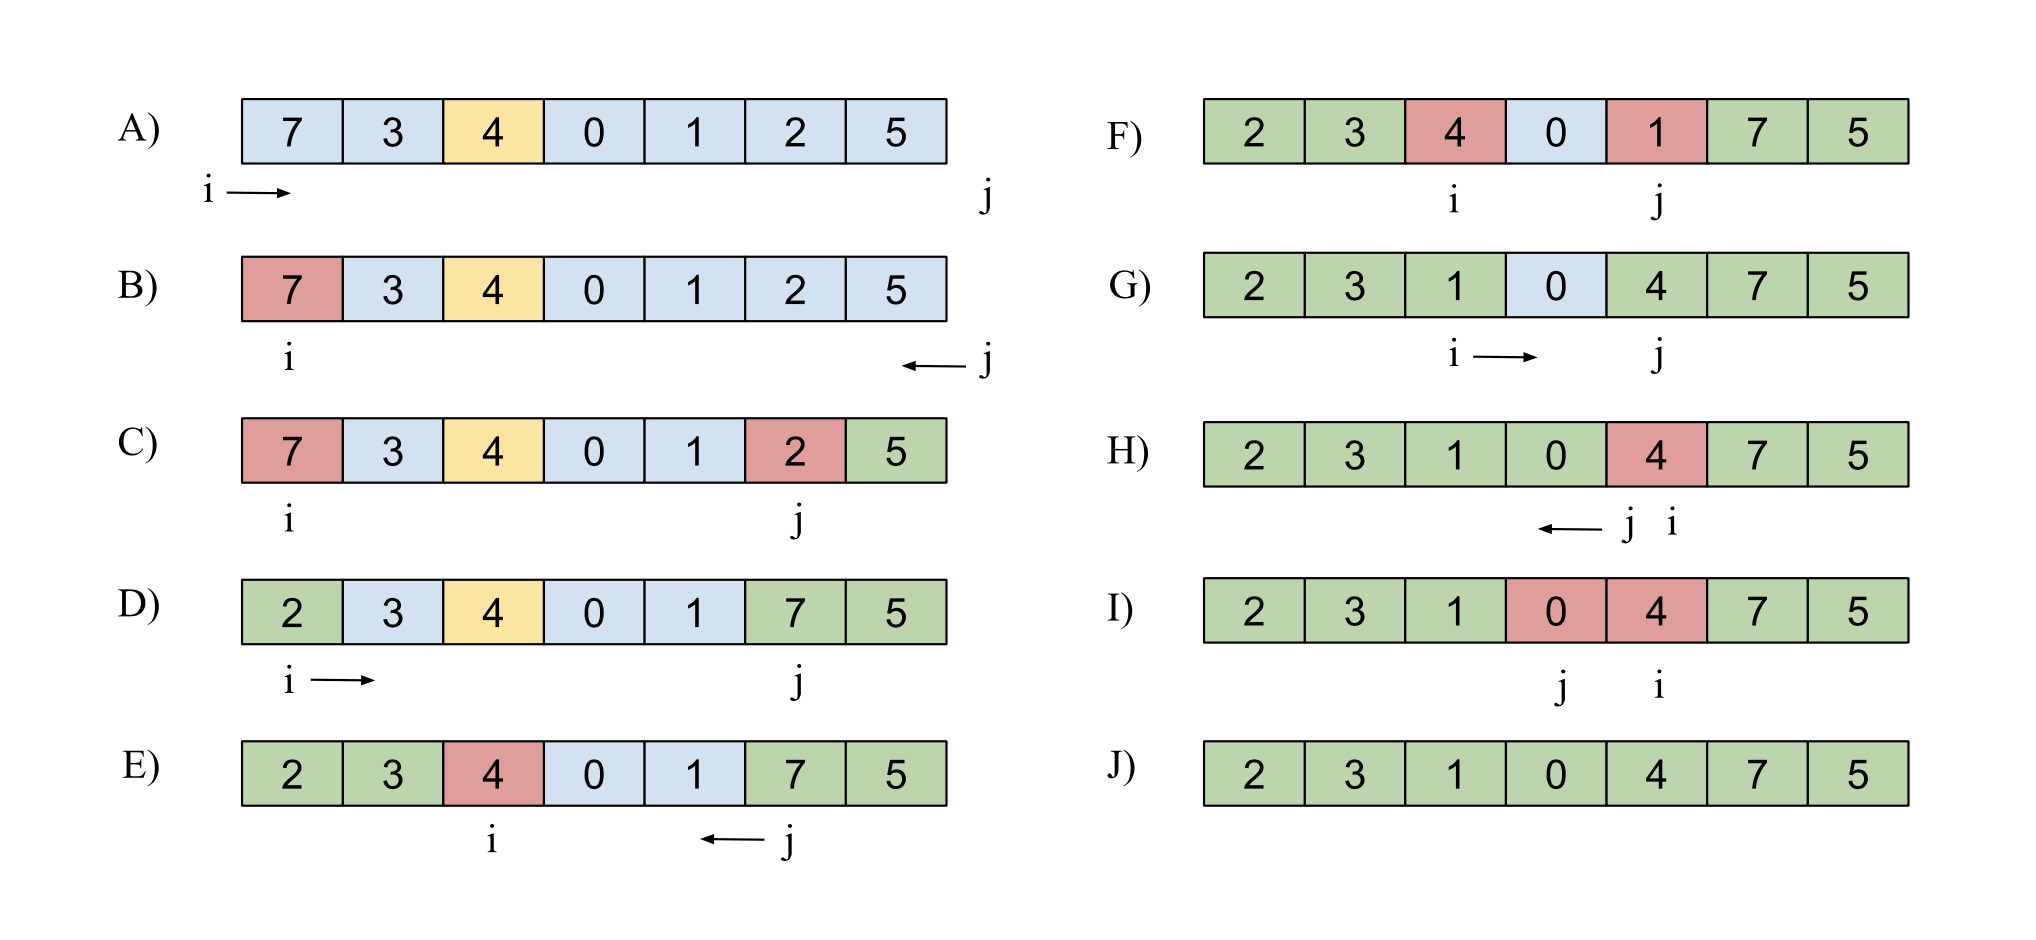
\includegraphics[scale=0.5]{img/pivot_partitioning.png}
  \end{center}
  \caption{A picture of the same tucan looking the other way!}
\end{figure}

 


\section{Complexity analysis}
\subsection{Worst-case analysis}
\subsection{Average-case analysis}
\subsection{Analysis of randomized Quicksort}

\section{Parallel processing}
\subsection{Scaling features}
\subsection{Parallelizing Quicksort}

\section{Computational geometry and the convex hull problem}
Computational geometry is the study of algorithms for the solution of geometric problems in the Euclidean space \cite{paper}.
The convex hull problem belongs to this class of problems, and has a wide range of applications across several disciplines
(e.g. data classification, collision avoidance, image processing and recognition). It is defined as follows:
given a set of points, find the smallest convex polygon containing all the points \cite{geowiki}.
For the purpose of this project, we will consider only the planar convex hull, with 2D Cartesian coordinates.

\subsection{The Quickhull algorithm}
The Quickhull algorithm is a variation of Quicksort for the solution of the convex hull problem.
The algorithms works as follows:
an initial partitioning step is done by picking the leftmost and rightmost point.
Let these two points be $p_1$ and $p_2$, respectively.
The line connecting $p_1$ and $p_2$ splits the set in two parts.
For each subset, we search for the farthest point from the line: let this point be $p_{max}$.
If it exists, the points lying inside the triangle $p_1p_2p_{max}$ are removed from the set,
and the recursive step is applied on the points that lie outside the lines $p_1p_{max}$ and $p_2p_{max}$.
Again, let $p_1$ and $p_2$ be the end points of the line in the recursive step.
The stop condition occurs when $p_{max}$ is not found, as there are no points outside $p_1p_2$.
The very first steps of the algorithm are illustrated in Figure \ref{fig:qh-steps}.
The pseudocode is given in Algorithms \ref{alg:qh1} and \ref{alg:qh2}.

\begin{figure}[H]
    \centering
    \begin{minipage}{.33\linewidth}
		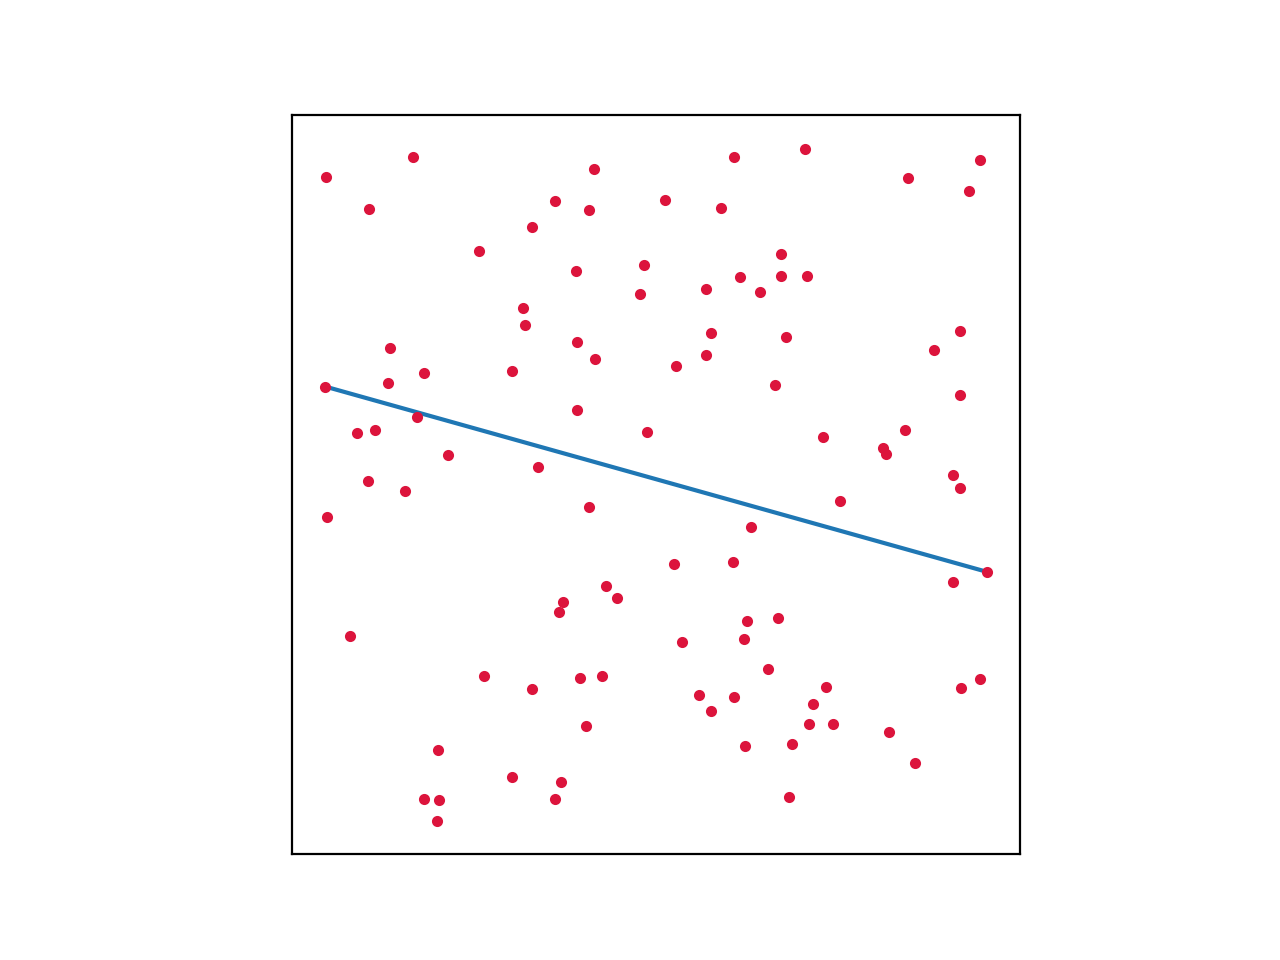
\includegraphics[width=\linewidth]{quickhull1.png}
	\end{minipage}
	\begin{minipage}{.33\linewidth}
		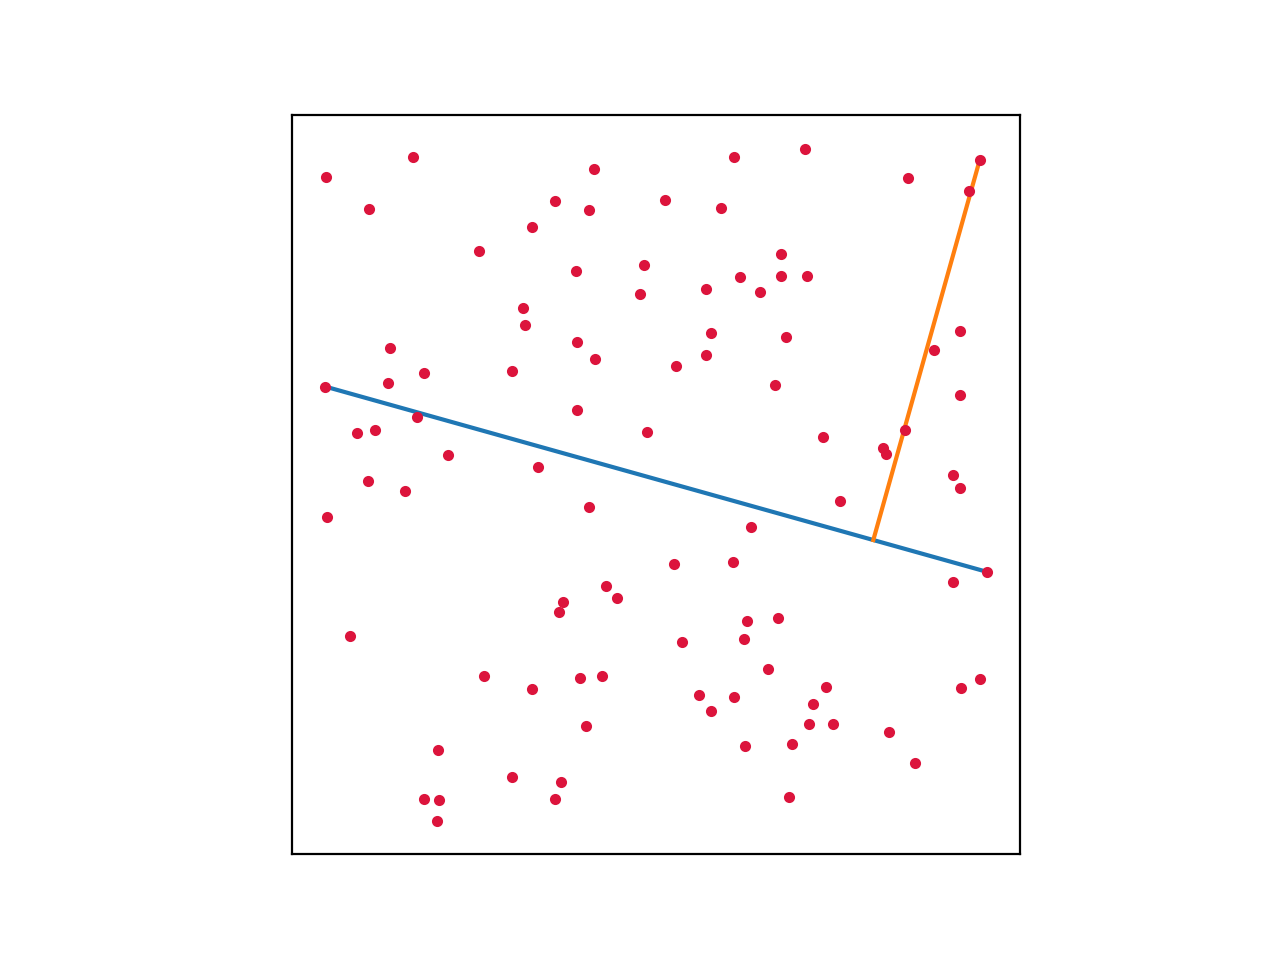
\includegraphics[width=\linewidth]{quickhull2.png}
	\end{minipage}
    \begin{minipage}{.33\linewidth}
		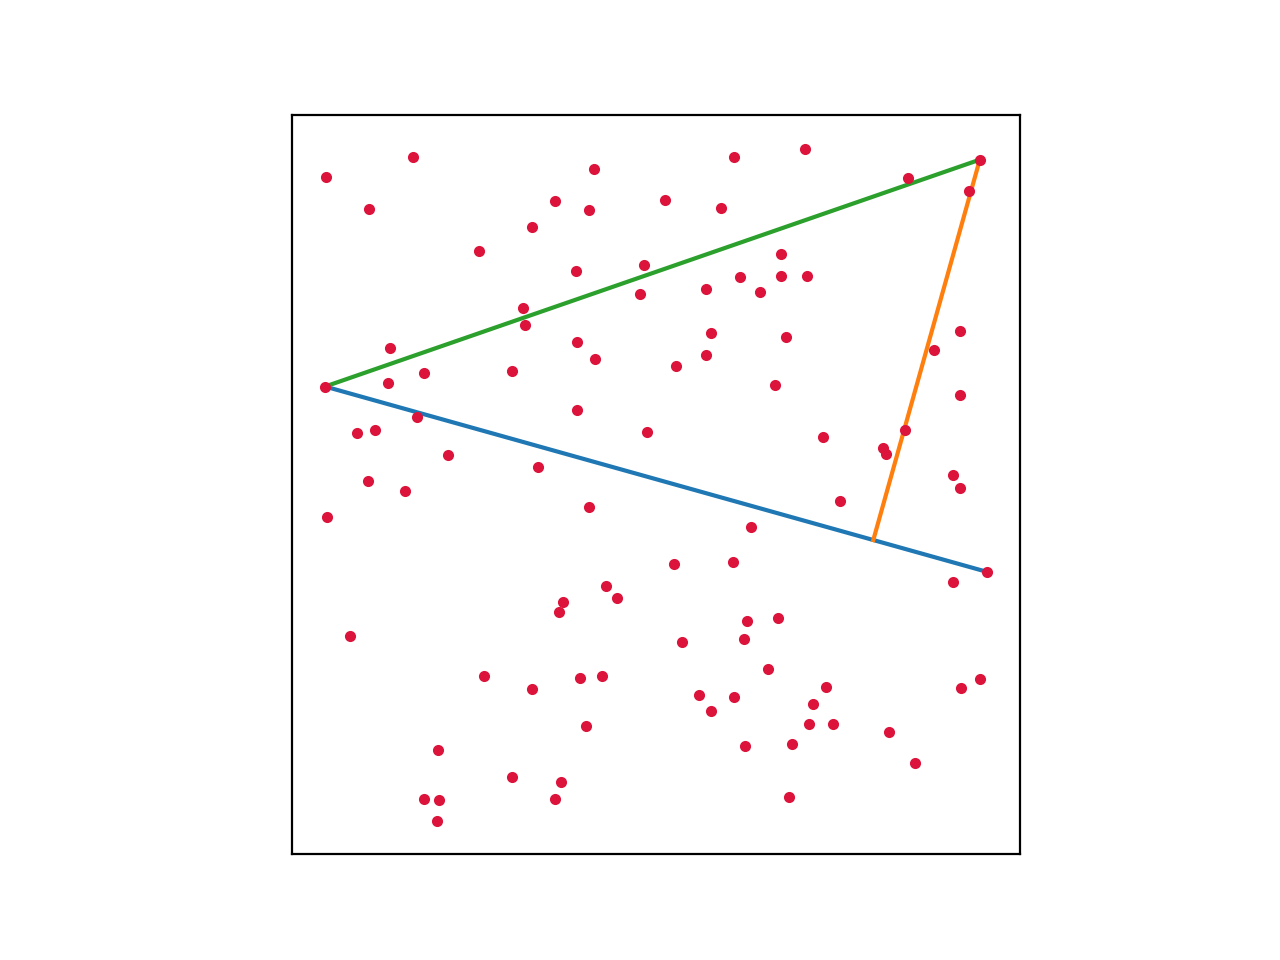
\includegraphics[width=\linewidth]{quickhull3.png}
	\end{minipage}
    \caption{Three steps of the Quickhull algorithm: the line $p_1p_2$ partitions the set of points in two subsets (left); the farthest point $p_{max}$ from the line is found (middle); the triangle $p_1p_2p_{max}$ shrinks the solution set (right).}
    \label{fig:qh-steps}
\end{figure}

\begin{algorithm}
    \caption{Quickhull ($P$)}
    \label{alg:qh1}
    P is a set of points with (x, y) coordinates

    Find the points $p_1$ and $p_2$ with x-coordinates $x_{min}$ and $x_{max}$

    Quickhull\_onside($P$, $p_1$, $p_2$, $1$)

    Quickhull\_onside($P$, $p_1$, $p_2$, $-1$)
\end{algorithm}
\begin{algorithm}
  \caption{Quickhull\_onside ($P$, $p_1$, $p_2$, $s$)}
  \label{alg:qh2}
  Let $p_{max}$ be the the point that is farthest from the line $p_1p_2$, on side $s$.

  \If(){$p_{max}$ does not exist}{return}

  Remove from $P$ all points that lie in the triangle $p_1p_2p_{max}$

  Let $s_1$ and $s_2$ be the outer sides of lines $p_1p_{max}$ and $p_2p_{max}$

  Quickhull\_onside($P$, $p_{max}$, $p_1$, $s_1$)

  Quickhull\_onside($P$, $p_{max}$, $p_2$, $s_2$)
\end{algorithm}

We can observe how Quickhull, just like Quicksort,
is both a divide-and-conquer and a sorting algorithm. The former approach is implemented by partitioning,
splitting the initial problem into smaller subproblems in a recursive fashion, whereas the latter is applied by comparing
Euclidean distances between points. Again, the complexity is $O(n^2)$ in the worst case and $O(n\log{n})$ in the average case.

\subsection{Distributed Quickhull}
The Quickhull algorithm is sequential by design,
as each recursive call depends on the previous ones for the computation of the solution set \cite{qhpaper}.
Therefore, parallelizing the algorithm by multithreading is not feasible, as it is not possible to independently compute the solution to subproblems.
However, the set of points can be distributed over multiple processes, and inter-process communication can be used to combine the partial results.\\
The pseudocode of the distributed version of Quickhull is given in Algorithm \ref{alg:qh3}.

\begin{algorithm}
  \caption{Distributed Quickhull ($P$)}
  \label{alg:qh3}
  Each process computes the points with minimum and maximum x-coordinate among their local portion of the dataset, then the global minimum and maximum are computed, and broadcast to all processes (\textit{allreduce}).

  Each process computes the farthest point from the line joining the two points, and the global result is found (\textit{allreduce}).

  Once each process has all three vertices of the triangle, they can remove the points that lie inside the triangle from their dataset.

  The recursive step is repeated just like in the sequential version.

  At the end, the solution is scattered over all processes, so it must be gathered on the root process (\textit{gather}).
\end{algorithm}

As we can see, the procedure is almost identical to the sequential version.
The key difference is the use of interprocess communication in the partitioning steps:
the computation performed by each process to find the leftmost and rightmost points, as well as the farthest point at every iteration,
is limited to a subset of points, so the results of all processes must be combined, in order to obtain the global result.
Note that communication is used just for the aforementioned purpose, and to combine the final solution on the root process,
keeping the communication cost low.

\subsubsection{Scaling analysis}
Running the algorithm for large input sizes with different numbers of processes, we can observe significant gains in performance.
A scaling chart is reported in Figure \ref{fig:qh-scaling}.
\begin{figure}[h!]
    \centering
    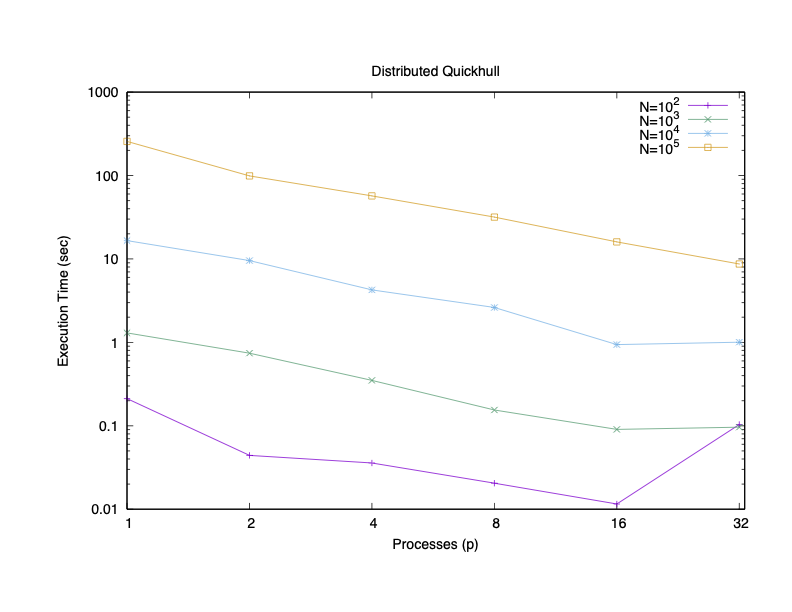
\includegraphics[width=0.6\linewidth]{gpStrongTime.png}
    \caption{Performance scaling of distributed Quickhull.}
    \label{fig:qh-scaling}
\end{figure}

We can observe the gain in performance obtained by the distributed version of the algorithm:
by doubling the number of processes, the execution time roughly halves.
However, we can also observe the effect of over-parallelizing with respect to the problem size:
e.g. for $N=10^2$, 32 processes perform worse than 16.

%%%%%
\clearpage
\bibliographystyle{abbrv}
\bibliography{references}



\end{document}